
\begin{figure}[h!]
\textbf{Tema d'Esame di Gennaio 2015}\\ \\
Calcolare il minimo coefficente di attrito statico tra asfalto e pneumatico in modo tale che un'auto che pesa $100kg$ riesca a percorrere una curva di raggio $850m$ a $60km/h$ senza sbandare
\begin{center}
		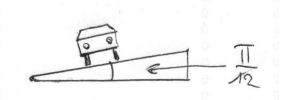
\includegraphics[scale=0.8]{ES1/FEB012015.jpg}
	\end{center}
\end{figure}

\begin{figure}[h!]
\textbf{Tema d'Esame di Febbraio 2015}\\ \\
 Calcolare la velocità massima alla quale un'automobile di $1 t$ può percorrere una curva di
raggio $900 m$ e inclinata di $\pi/12$ sapendo che il coefficiente di attrito statico tra asfalto e
pneumatico è $0.5$
\end{figure}

\begin{figure}[h!]
\textbf{Tema d'Esame di Giugno 2015}\\ \\
Calcolare il minimo coefficente di attrito statico tra un corpo di massa $3kg$ e il piano inclinato sui cui è appoggiato in modo che inclinando il piano di $45^{\circ}$ il corpo rimanga fermo
\end{figure}

\begin{figure}[h!]
\textbf{Tema d'Esame di Luglio 2015}\\ \\
Un elicottero vola orizzontalmente a $200km/h$ e a una quota di $500m$ lancia un carico che deve toccare terra in un punto ben preciso. Trascurando la resistenza dell'aria a quale distanza orizzontale dal bersaglio l'equipaggio deve effettuare il lancio?
\end{figure}

\begin{figure}[h!]
\textbf{Tema d'Esame di Luglio 2015}\\ \\
Calcolare l'angolo massimo a cui si può inclinare un piano su cui è appoggiato un corpo di massa $5kg$ per cui il corpo rimane fermo. Il coefficente di attrito statico tra un corpo è $0.9$.
\end{figure}


